\section{Assessing the Performance Impact}

\label{sec:predictimprove}
%\todo{Adding a picture, maybe similar to Sammati paper}
%\todo{memory bound. Predict memory bound. IO we can't bound. original 100, we remove 80. Latency can be predict to the execution time.  } 
Fixing false sharing does not necessarily yield significant performance speedups, even for instances with a large number of cache invalidations~\cite{Sheriff, Predator}. Zhao et al. even observes that fixing false sharing may even slow down a program, since padding data structures may increase its memory footprint or lose cache locality~\cite{qinzhao}. Thus, it is very important to rule out insignificant false sharing instances, which are not false-positives, yet reporting them increases the manual burden for fixes.

\cheetah{} makes the first attempt to quantitatively assess the potential performance gain of fixing a false sharing instance based on the results of an execution. We agree that different executions may vary on the specific details, but this should not change the overall prediction result: whether a false sharing instance is significant or not. Actually, the evaluation described in Section~\ref{sec:precision} confirms that our predicted performance has less than a 10\% difference from that of the actual fixes. Based on this prediction, programmers can focus on severe problems only, avoiding unnecessary manual effort spent on insignificant cases.

\cheetah{}'s assessment is based on the following observations:

\begin{itemize}
\item {\bf Observation 1:} Samples are evenly distributed over the whole execution. Based on this, we can use the sampling technique to represent the whole execution. The similar idea has been widely used by prior work, such as Oprofile~\cite{oprofile} and Gprof~\cite{DBLP:conf/sigplan/GrahamKM82} to identify the hotspots of function calls.

\item {\bf Observation 2:} The PMU provides the latency information (e.g. cycles) of each memory access; the latency of memory accesses with false sharing are significantly higher than that of other accesses. 

\end{itemize}

Based on these two observations, we propose to use the sampled cycles to represent the whole execution, and further predict the performance impact of falsely-shared objects by replacing these cycles with the average cycles of memory accesses without false sharing. The assessment is performed in three steps, listed as follows: 

\begin{itemize}
\item \cheetah{} first predicts the possible cycles after fixes by replacing actual cycles with the average cycles of memory accesses without false sharing, as discussed in Section~\ref{sec:impactobject}. 

\item Then, \cheetah{} assesses the performance impact of fixes on the related threads, which is discussed in Section~\ref{sec:impactthread}. 
 
\item In the end, \cheetah{} assesses the performance impact on the application in Section~\ref{sec:impactapp}. 
\end{itemize}

The remainder of this section discusses the detailed assessment step-by-step. For reasons of simplicity, we abbreviate the falsely-shared object as ``$O$'', the related thread as ``$t$'', the prediction as ``$Pred$'', the runtime as ``$RT$'', and the application as ``$App$''. 

\subsection{Impact on Accesses to the Object}
\label{sec:impactobject}

At first, \cheetah{} predicts the possible cycles of accesses after fixing false sharing of the object $O$. \cheetah{} tracks the number of cycles and accesses on each word, thus it is convenient to compute the total cycles of accesses --- $Cycles\_O$, and the total number of accesses --- $Accesses\_O$, on a specific object $O$.  

However, it is impossible to know the average cycles of every access after fixing --- $AverCycles\_{nofs}$, without actual fixes ({\it \cheetah{} utilizes the average cycles in serial phases ($AverCycles\_{serial}$) to approximate this value}). There is no false sharing in serial phases, and $AverCycles\_{serial}$ represents the least number of cycles for memory accesses after fixes. If \cheetah{} does not track any accesses in serial phases, a default value learned from experience will be utilized as $AverCycles\_{serial}$. In reality, $AverCycles\_{nofs}$ can be larger than $AverCycles\_{serial}$, since fixing false sharing may lead to excessive memory consumption or the loss of locality~\cite{qinzhao}. \cheetah{} actually predicts the best performance of fixing a false sharing instance. 
 
\cheetah{} computes the total cycles of accesses after fixes ($PredCycles\_{O}$) based on the EQ.(\ref{eq:predictedcyclesofo}).  It is expected that $PredCycles\_{O}$ will be less than the total cycles before fixing --- $Cycles_O$, since fixing a false sharing problem will reduce the execution time and cycles.  

\begin{equation}
\label{eq:predictedcyclesofo}
PredCycles\_{O} = (AverCycles\_{nofs} * Accesses\_O)
\end{equation} 

\subsection{Impact on Related Threads}
\label{sec:impactthread}

The second step is to assess how reducing the access cycles of $O$ ($PredCycles\_{O}$) can potentially affect the execution time of its related threads. 

\Cheetah{} collects the following runtime information of every thread: the execution time --- $RT\_{t}$, the total number of accesses --- $Accesses\_{t}$, and the total cycles of all memory accesses --- $Cycles\_{t}$. In order to avoid any lookup overhead, \cheetah{} lets every thread handle the sample events of the current thread, and records the corresponding number of accesses and cycles. To collect $RT\_{t}$, \cheetah{} intercepts the creation of threads by passing a custom function as the start routine. \cheetah{} acquires the timestamp before and after the execution of a thread using the RDTSC (ReaD-Time Stamp Counter)~\cite{rtdsc}, and regards the difference to be the execution time of a particular thread. In current implementation, we do not take into account the waiting time of different threads caused by synchronizations; we leave this for future work. 
%To gather the number of accesses and cycles of every thread, \cheetah{} makes every thread to respond the signal handler and records the number of accesses and cycles correspondingly. 

After the collection, \cheetah{} predicts the cycles of every related thread --- $PredCycles\_{t}$ --- after fixes as the EQ.(\ref{eq:predictedcyclesofthread}). 

\begin{equation}
\label{eq:predictedcyclesofthread}
 PredCycles\_{t} = Cycles\_{t} - Cycles\_{O} + PredCycles\_{O} 
\end{equation} 
 
Based on $PredCycles\_{t}$, \cheetah{} assesses the predicted runtime of a thread --- $PredRT_{t}$ --- as the EQ.(\ref{eq:predictedrtofthread}). We assume that {\bf the execution time is proportional to the cycles of accesses}, such that fewer cycles indicates less execution time, and corresponds to a performance speedup. It is expected that fixing the false sharing problem inside the object $O$ will improve the performance for its related threads, with less $PredCycles\_{t}$ and $PredRT_{t}$. 

\begin{equation}
\label{eq:predictedrtofthread}
 PredRT\_{t} = (PredCycles\_{t} / Cycles\_{t}) * RT\_{t} 
\end{equation} 

\subsection{Impact on the Application}
\label{sec:impactapp}

In the end, \cheetah{} assesses how fixes will change the performance of the application. 

Actually, improving the performance of a thread may not increase the final performance of an application if this thread is not in the critical path.  To simplify the prediction, as well as verify our idea, \cheetah{} currently focuses on applications with the normal fork-join model shown as Figure~\ref{fig:forkjoinmodel}. This model is the most important and widely-used model in actuality. All applications that we have evaluated in this paper utilize this fork-join model. The performance assessment will be more complicated if nested threads are utilized inside an application. 


\begin{figure*}[ht!]
\begin{center}
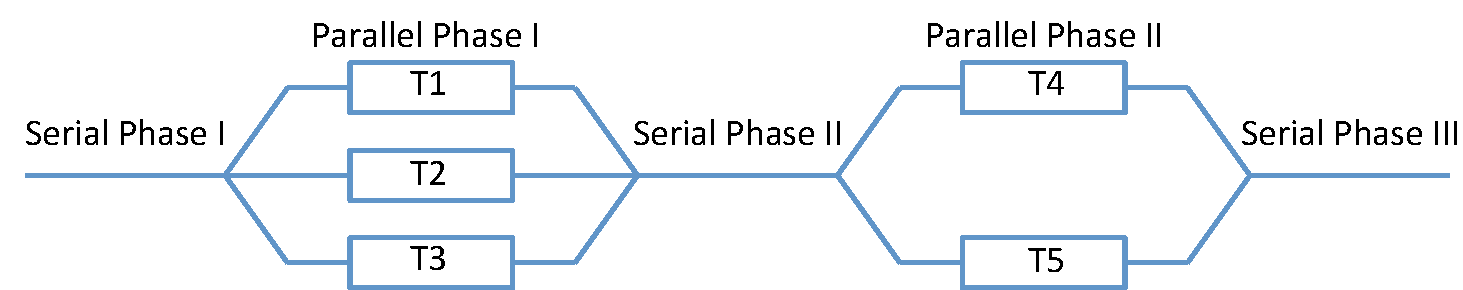
\includegraphics[width=6in]{figure/forkjoin}
\end{center}
\caption{The fork-join model, currently supported by \Cheetah{} to assess the performance impact of false sharing instances. }
\label{fig:forkjoinmodel}
\end{figure*}

\cheetah{} tracks the creations and joins of threads in order to verify whether an application belongs to the fork-join model or not. \Cheetah{} also collects the execution time of different serial and parallel phases, using RDTSC (ReaD-Time Stamp Counter) available on X86 machines~\cite{rtdsc}. In the fork-join model, shown in Figure~\ref{fig:forkjoinmodel}, an application leaves a serial phase after the creation of a thread; it leaves a parallel phase after all child threads (created in the current phase) have been successfully joined. 

Based on the runtime information of every parallel and serial phase, \cheetah{} assesses the final performance impact by recomputing the length of each phase, and the total time after fixing. The length of each phase is decided by the thread with the longest execution time, while the total time of an application is equal to the sum of different parallel and serial phases. 

After \cheetah{} computes the possible execution time of an application after fixing a false sharing problem, \cheetah{} will compute and report the potential performance improvement of every falsely-shared object, based on EQ.(\ref{eq:improvement}). Then, programmers can focus on those with the most serious performance impact. We further verify the precision of \cheetah{}'s assessment in Section~\ref{sec:precision}.

\begin{equation}
\label{eq:improvement}
PerfImprove = RT\_{App} / PredRT\_{App}
\end{equation}

%We will uses an example to show that. For example, there is a false sharing problem that will involved in the $T1$ and $T2$ of Figure~\ref{fig:forkjoinmodel}, but not other threads.  We will assess the possible runtime of $PredictRT_{T1}$ and $PredictRT_{T2}$. Then we checked that whether these predicted runtime will affect the runtime of parallel phase I by checking whether these two runtime are less than the runtime of $T3$ at first. If it won't, then fixing the false sharing problem won't affect the final performance. Otherwise, we have to recompute the length of parallel phase I, while the length of other phases will keep the same. By doing that, we will get a new runtime for the application. Using the EQ.(\ref{eq:improvement}), we can compute the potential performance improvement of this application by fixing the false sharing problems related to the thread $T1$ and $T2$. 









